%%%%%%%%%%%%%%%%%%%%%%%%%%%%%%%%%%%%%%%%%%%%%%%%%%%%%%%%%%%%%%%%%%%%%%%%%%
%% Review Volume (last updated on 2014/03/05) %%
%% Trim Size: 9.61in x 6.69in %%
%% Text Area: 8in (include runningheads) x 5in %%
%% Main Text: 10 on 13pt %%
%% For support: Yolande Koh, <ykoh@wspc.com.sg> %%
%% D. Rajesh Babu, <rajesh@wspc.com.sg> %%
%%%%%%%%%%%%%%%%%%%%%%%%%%%%%%%%%%%%%%%%%%%%%%%%%%%%%%%%%%%%%%%%%%%%%%%%%%
%%
%\documentclass[wsdraft]{ws-rv961x669} % to draw border line around text area
%\documentclass{ws-rv961x669}
\documentclass[addchapnum]{ws-rv961x669} % to add chapter number in volume
\usepackage{ws-rv-van} % numbered citation/references (default)
%\usepackage{ws-rv-thm} % comment this line when `amsthm / theorem / ntheorem` package is used
%\usepackage{subfigure} % required only when side-by-side / subfigures are used
\usepackage{ws-index} % required only when multiple indexes are used
%\usepackage[colorlinks=false]{hyperref}
%\usepackage{doi}
\usepackage{bbm}
\usepackage{amsmath}
\usepackage{amssymb}
\makeindex
\newindex{aindx}{adx}{and}{Author Index} % author index
\renewindex{default}{idx}{ind}{Subject Index} % subject index

\newcommand{\req}[1]{Eq.~(\ref{#1})}
 
\begin{document}

\chapter[Dynamics flavor mixing through transition moments]{Dynamics flavor mixing through transition moments\label{JR_ch1}}

\author[J. Rafelski and A. Steinmetz]{Johann Rafelski and Andrew Steinmetz\footnote{JohannR@Arizona.EDU,AJSteinmetz@Arizona.EDU}}
\aindx{Rafelski, J.}
\aindx{Steinmetz, A.}

\address{Department of Physics, The University of Arizona, Tucson, AZ 85721, USA}

\begin{abstract} 
As neutrinos are naturally massless in the standard model the observed flavor oscillation presents a problem. Moreover it is unknown if neutrinos are Dirac-type or Majorana-type fermions. We show that the required neutrino flavor mixing can be driven by electromagnetic transition dipole moment. We  analyze sensitivity of the Pontecorvo–Maki–Nakagawa–Sakata (PMNS) matrix to strong electromagnetic fields.
\end{abstract}

\markboth{Johann Rafelski and Andrew Steinmetz}{Neutrinos in EM fields} % Customized running heads

\body

%\tableofcontents\

%%%%%%%%%%%%%%%%%%%%%%%%%%%%%%%%%%%%
\section{Introduction}
\label{sec:intro}
%%%%%%%%%%%%%%%%%%%%%%%%%%%%%%%%%%%%
\noindent 
In this work we look at the connection between the magnetic dipole (transition) moments of neutrinos~\cite{Shrock:1980vy} and neutrino flavor oscillations. Neutrinos once were the dominant form of energy density in the universe~\cite{Rafelski:2023emw}. Aside of their importance in the context of  of stellar evolution and Super Novea, there is profound interest in understanding their physical properties due to their importance as a bridge to beyond standard model (BSM) physics. Their electromagnetic (EM) properties have been considered before~\cite{Giunti:2014ixa} but to best of our knowledge this is a first consideration of EM contribution to flavor oscillation.  

The size of the neutrino magnetic dipole moment is relatively small with a lower bound determined by the standard model and an upper bound from reactor or solar observations given by~\citep{Studenikin:2016ykv,Canas:2015yoa,AristizabalSierra:2021fuc}
\begin{align}
    \label{momentbound:1}
    10^{-19}\mu_{B}<\mu_{\nu}^\mathrm{eff}<10^{-10}\mu_{B}\,,\qquad\mu_{B}=\frac{e\hbar}{2m}
\end{align}
where $\mu_{B}$ is the Bohr magneton and $\mu_{\nu}^\mathrm{eff}$ is the effective and characteristic size of the neutrino magnetic moment.

Considering higher order diagrams neutrino should manifestation non-minimal EM interactions~\citep{Shrock:1980vy,DUNE:2020fgq} of the form
\begin{gather}
    \label{mu:1}
\boldsymbol{\mu}=\mu_{\ell\ell'}=
	\begin{pmatrix}
		\mu_{ee} & \mu_{e\mu} & \mu_{e\tau} \\
		\mu_{e\mu}^{*} & \mu_{\mu\mu} & \mu_{\mu\tau} \\
		\mu_{e\tau}^{*} & \mu_{\mu\tau}^{*} & \mu_{\tau\tau}\,,
	\end{pmatrix}
\end{gather}
where $\ell$ are the neutral lepton flavor indices $\ell\in\nu_{e},\nu_{\mu},\nu_{\tau}$. The transition moments are small~\cite{Shrock:1980vy} but  Beyond Standard Model (BSM) physics is capable to produce an abnormally large electromagnetic dipole~\citep{Lindner:2017uvt,Brdar:2020quo} within the bounds of~\req{momentbound:1} which may manifest itself in strong field or/and dense matter environments.

%%%%%%%%%%%%%%%%%%%%%%%%%%%%%%%%%%%%%%%
\section{Description of neutrino flavor mixing}
\label{sec:numass}
%%%%%%%%%%%%%%%%%%%%%%%%%%%%%
Experiment shows that neutrino mass and flavor eigenstates differ. This misalignment between the two representations is described as rotation of the neutrino flavor 3-vector where $N=3$ is the number of generations. The unitary mixing matrix $V_{\ell k}$ allowing the change of basis between mass and flavor eigenstates is 
\begin{alignat}{1}
	\label{basis:1} \nu_{\ell}=\sum_{k=1}^{3}V_{\ell k}\nu_{k}\,\rightarrow
	\begin{pmatrix}
		\nu_{e}\\
		\nu_{\mu}\\
		\nu_{\tau}
	\end{pmatrix}=
	\begin{pmatrix}
		V_{e1} & V_{e2} & V_{e3}\\
		V_{\mu1} & V_{\mu2} & V_{\mu3}\\
		V_{\tau1} & V_{\tau2} & V_{\tau3}
	\end{pmatrix}
	\begin{pmatrix}
		\nu_{1}\\
		\nu_{2}\\
		\nu_{3}
	\end{pmatrix}\,,
\end{alignat}
where $\nu_{\ell}$ is the neutrino state vector written in the flavor basis while in the mass basis we use $\nu_{k}$ with $k\in1,2,3$. Hereafter we will use implied summation  over repeated indices.

The parametrization of component of the mixing matrix depends on the Dirac- or Majorana-nature of the neutrinos.  Consider $U_{\ell\ell'}$ to be the Dirac  neutrino matrix. In the standard parameterization~\citep{Schwartz:2014sze}, the PMNS rotation matrix $U_{\ell k}$ can be expressed as
\begin{alignat}{1}
	\label{rotation:1} U_{\ell k} =
	  \begin{pmatrix}
		  c_{12}c_{13} & s_{12}c_{13} & s_{13}e^{-i\delta}\\
		  -s_{12}c_{23} - c_{12}s_{13}s_{23}e^{i\delta} & c_{12}c_{23} - s_{12}s_{13}s_{23}e^{i\delta} & c_{13}s_{23}\\
		  s_{12}s_{23} - c_{12}s_{13}c_{23}e^{i\delta}& -c_{12}s_{23} - s_{12}s_{13}c_{23}e^{i\delta} & c_{13}c_{23}
	  \end{pmatrix}\,,
\end{alignat}
where $c_{ij} = \mathrm{cos}(\theta_{ij})$ and $s_{ij} = \mathrm{sin}(\theta_{ij})$. In this convention, the three mixing angles $(\theta_{12}, \theta_{13}, \theta_{23})$, are understood to be the Euler angles for generalized rotations. 

For the Majorana case of interest to us we must allow a greater number of complex phases described by additional matrix $P$
\begin{alignat}{1}
	\label{phases:1} &V_{\ell k} = U_{\ell k'}P_{k'k}\,,\\
	\label{phases:3} &P_{kk'} = \mathrm{diag}(e^{i\rho},e^{i\sigma},1)\,.
\end{alignat}
Majorana neutrinos allow up to two additional complex phases $\rho$ and $\sigma$ which along with $\delta$ participate in CP-violation. The mixing matrix defined in \req{phases:1} can then be used to diagonalize the mass matrix $M_{\ell\ell'}$ from the flavor basis into the mass basis as
\begin{align}
    \label{diag:1}
    V_{\ell k}^{\dag}M_{\ell\ell'}V_{\ell'k'} = M_{kk'} = \mathrm{diag}(m_{1},m_{2},m_{3})\,.
\end{align}

The Majorana mass Lagrangian in the flavor basis is written as
\begin{alignat}{1}
	\label{mass:1} -\mathcal{L}_{\mathrm{mass}}^{\mathrm{Maj.}}=\frac{1}{2}\bar\nu_{\ell}^{L}M_{\ell\ell'}\left(\nu_{\ell'}^{L}\right)^{c}+\mathrm{h.c}\,,
\end{alignat}
where $\nu^{L}$ refers to left-handed chiral states which can be obtained using projection operators and $\gamma^{5}$. Bars atop vectors represent the Dirac adjoint in the usual manner. The superscript $\nu^{c}$ refers to the charge conjugated state. \req{phases:1} can then diagonalize mass matrix $M_{\ell\ell'}\rightarrow M_{kk'}$ to real positive masses.

For Majorana neutrinos, the states can be reorganized into
\begin{align}
    \label{maj:1}
    \nu_{\ell} = \nu_{\ell}^{L}+\left(\nu_{\ell}^{L}\right)^{c}\,,\qquad
    \nu=\nu^{c}\,
\end{align}
which lets us recast \req{mass:1} as in either flavor or mass basis
\begin{gather}
    \label{mass:2}
    \mathcal{L}_{\mathrm{mass}}^{\mathrm{Maj.}}=\frac{1}{2}\nu_{\ell}^{T}C^{\dag}M_{\ell\ell'}\nu_{\ell'}+\mathrm{h.c}\,,\\
    \nu_{\ell} = V_{\ell k}\nu_{k}\,,\qquad V_{\ell k}^{T}M_{\ell\ell'}V_{\ell'k'}=M_{kk'}\,.
\end{gather}

%%%%%%%%%%%%%%%%%%%%%%%%%%%%%%%%%%%%%%%
\section{Introducing electromagnetic fields to neutrino dynamics}
\label{sec:numoment}
%%%%%%%%%%%%%%%%%%%%%%%%%%%%%%%%%%%%%%%
\noindent As neutrinos are electrically neutral, they have no intrinsic magnetic moment due to their spin, therefore any magnetic moment present is considered anomalous. A small anomalous magnetic moment (AMM) can be introduced into the Lagrangian~\citep{Itzykson:1980rh,Steinmetz:2018ryf} for the neutrino via a Pauli term. As our focus is on effective field theories, we will not worry with the fact that the Pauli Lagrangian is 5-Dimensional and thus fails to be renormalizable. The Pauli Lagrangian for the AMM for Majorana-like neutrinos in the flavor basis is given by
\begin{align}
	\label{moment:1} \mathcal{L}_{\mathrm{AMM}}^\mathrm{Maj.}=\frac{1}{2}\nu_{\ell}^{T}C^{\dag}\left(\mu_{\ell\ell'}\frac{i}{2}\gamma_{\alpha}\gamma_{\beta}F^{\alpha\beta}\right)\nu_{\ell'}+\mathrm{h.c.}
\end{align}
The matrix $\mu_{\ell\ell'}$ are the AMM couplings given in \req{mu:1} and $F^{\alpha\beta}$ is the standard electromagnetic field tensor.

Because of CPT considerations, Majorana neutrino are forbidden diagonal magnetic moments and can only have off-diagonal transition moments. The trace of $\mu_{\ell\ell'}$ is zero thus all the diagonal elements are identically zero. Since transition AMM elements serve to break lepton number conservation allowing for $\nu_{\ell}+\gamma\rightarrow\nu_{\ell'}$ processes, it suggests than neutrinos could be \lq\lq remixed\rq\rq\ when exposed to strong electrodynamic fields similar to remixing within matter in the Mikheyev-Smirnov-Wolfenstein (MSW) effect~\citep{Wolfenstein:1977ue,Mikheyev:1985zog,Bethe:1986ej,greiner2009gauge}. We note that such couplings are also possible for dark-sector physics if neutrinos coupled to a yet unknown vector field.

Majorana neutrinos have the following properties~\cite{Shrock:1982sc}
\begin{alignat}{1}
	\label{props:1}	M_{\ell\ell'}^{T}=M_{\ell\ell'}\,,\qquad
    \mu_{\ell\ell'}^{\dag}=\mu_{\ell\ell'}\,,\qquad
    \mu_{\ell\ell'}^{T}=-\mu_{\ell\ell'}\,,
\end{alignat}
such that the mass matrix $M_{\ell\ell'}$ is complex and symmetric while the moment matrix $\mu_{\ell\ell'}$ is Hermitian and fully anti-symmetric. This requires that the transitional magnetic moment elements are purely imaginary. We can combine the AMM contribution and the mass term in~\req{mass:1} and~\req{moment:1} to write an effective Lagrangian containing both terms as
\begin{align}
	\label{massmom:1}
    \mathcal{L}_\mathrm{eff}^\mathrm{Maj.} =
    \mathcal{L}_\mathrm{mass}^\mathrm{Maj.} + \mathcal{L}_\mathrm{AMM}^\mathrm{Maj.} = 
    \frac{1}{2}\nu_{\ell}^{T}C^{\dag}\left(M_{\ell\ell'}+\mu_{\ell\ell'}\frac{i}{2}\gamma_{\alpha}\gamma_{\beta}F^{\alpha\beta}\right)\nu_{\ell'}+\mathrm{h.c.}
\end{align}
We define the generalized mass-dipole matrix $\mathcal{M}_{\ell\ell'}$ present in \req{massmom:1} as
\begin{align}
	\label{massmom:2}
    \mathcal{M}_{\ell\ell'}(\vec{E},\vec{B})\equiv M_{\ell\ell'}+\mu_{\ell\ell'}\frac{i}{2}\gamma_{\alpha}\gamma_{\beta}F^{\alpha\beta}\,.
\end{align}
Our goal in the following section will be to diagonalize this matrix as the freely propagating eigenstates of neutrinos within an electromagnetic field.

Further, we can understand the mass matrix (in the flavor basis) as a diagonal part and traceless part
\begin{align}
	\label{massmom:3}
    M_{\ell\ell'}=m_{\ell\ell'}^\mathrm{diag}+K_{\ell\ell'}\,,\qquad
    m_{\ell\ell'}^\mathrm{diag}=\mathrm{diag}(m_{\nu_{e}},m_{\nu_{\mu}},m_{\nu_{\tau}})\,,\qquad
    \mathrm{Tr}\left[K_{\ell\ell'}\right] = 0 \,,
\end{align}
where $m_{\ell\ell'}^\mathrm{diag}$ is the intrinsic flavor masses and $K_{\ell\ell'}$ is the off-diagonal interaction coupling between flavors prescribed by BSM physics. 

Since neutrino oscillation is experimentally verified, the coupling matrix cannot be fully zero, though elements of the intrinsic flavor masses can. The conditions for $K_{\ell\ell'}$ can be further constrained by group symmetry such as flavor SU(3). While non-Hermitian moments and group structure raise interesting possibilities, we will not explore them further here.

%%%%%%%%%%%%%%%%%%%%%%%%%%%%%%%%%%%%%%%
\section{Magnetic moment-flavor mixing for two generations}
\label{sec:mix}
%%%%%%%%%%%%%%%%%%%%%%%%%%%%%%%%%%%%%%%
\noindent To demonstrate an example of how spin (and thus magnetic moment) and flavor may mix, let us consider two generations of neutrinos for illustration. From the experimental data on neutrino oscillations, is is understood that either the two heavier (normal hierarchy) or the two lighter (inverted hierarchy) neutrino states are close together in mass. If the electromagnetic properties of the neutrino do indeed lead to flavor mixing effects, then it is likely the closer pair of neutrino mass states are most sensitive to the phenomenon.

It is still unknown which hierarchy neutrinos follow, therefore probing the EM properties of neutrinos may provide evidence for one model over the other. The behavior of the two generation neutrino model may then be valuable for subtle EM mixing effects especially in regard to the two neutrinos with more similar masses.

Following the notation established in \req{massmom:2} and \req{massmom:3} we write down the two-generation mass and dipole matrices as
\begin{alignat}{1}
	\label{mix:1} m_{\ell\ell'}^\mathrm{diag}= 
	\begin{pmatrix}
		m_{1} & 0\\
		0 & m_{2}
	\end{pmatrix}\,,\qquad
	K_{\ell\ell'} = 
	\begin{pmatrix}
		0 & m_{12}\\
		m_{12} & 0
	\end{pmatrix}\,,\qquad
	\mu_{\ell\ell'} = 
	\begin{pmatrix}
		0 & i\mu\\
		-i\mu & 0
	\end{pmatrix}\,.
\end{alignat}
If we take the mass matrix $M_{\ell\ell'}$ to be Hermitian $M_{\ell\ell'}^{\dag}=M_{\ell\ell'}$, this requires that all elements be full real. We also evaluate the $\gamma_{\alpha}\gamma_{\beta}F^{\alpha\beta}$ for pure magnetic fields in the Chiral basis yielding
\begin{align}
    \label{chiral:1}
    \frac{i}{2}\gamma_{\alpha}\gamma_{\beta}F^{\alpha\beta}=\mathbbm{1}_{2}\otimes\vec{\sigma}\cdot\vec{B}\,,
\end{align}
Suppressing the $2\times2$ identity matrix $\mathbbm{1}_{2}$, the overall mass-dipole matrix is then
\begin{alignat}{1}
	\label{mix:2} \mathcal{M}_{\ell\ell'} = 
	\begin{pmatrix}
		m_{1} & m_{12}+i\mu\vec{\sigma}\cdot\vec{B}\\
		m_{12}-i\mu\vec{\sigma}\cdot\vec{B} & m_{2}
	\end{pmatrix}\,,\ 
\end{alignat}

We introduce the concept of a `mass-dipole' eigenstate $\tilde{m}(E,B)$ resulting from a rotation $W_{\ell k}(\theta)$ which completely diagonalizes $\mathcal{M}_{\ell\ell'}$. This represents a unique basis that is distinct from the mass basis and the flavor basis. Since we have only two neutrino flavors, this rotation mixing matrix
\begin{alignat}{1}
	\label{mix:4} W_{\ell k}(\theta) = 
	\begin{pmatrix}
		\cos{\theta} & -\sin{\theta}\\
		\sin{\theta} & \cos{\theta}
	\end{pmatrix}
\end{alignat}
The mass-dipole diagonalization is then given by
\begin{alignat}{1}
	\label{mix:5} \tilde{m}_{kk'} = \mathrm{diag}(\tilde{m}_{1},\tilde{m}_{2})=W_{\ell k}^{T}\mathcal{M}_{\ell\ell'}W_{\ell'k'}
\end{alignat}
The eigenvalues of the mass-dipole matrix described in \req{mix:2} are therefore
\begin{align}
    \label{eigenvalue:1}
    \tilde{m}(B)_{\pm}=\frac{1}{2}\left(m_{2}+m_{2}\pm\sqrt{(m_{2}-m_{1})^{2}+4\left\rvert m_{12}\right\rvert^{2}+4\mu^{2}B^{2}}\right)
\end{align}

%%%%%%%%%%%%%%%%%%%%%%%%%%%%%%%%%%%%
\section*{Acknowledgements}
Harald Fritzsch enjoyed the US-South-West. On the way between Caltech and the Santa Fe Institute he sometimes made a stop at the half-way point, Tucson. On such occasions he explored Arizona mountains and  deserts; Figure\,\ref{Fig:AZcolloq2007} is showing our outing on occasion of March 23, 2007 physics colloquium at the University of Arizona: Harald was an avid observer and photographer of the desert fauna and flora. 
 
\begin{figure}%[hb]
\centerline{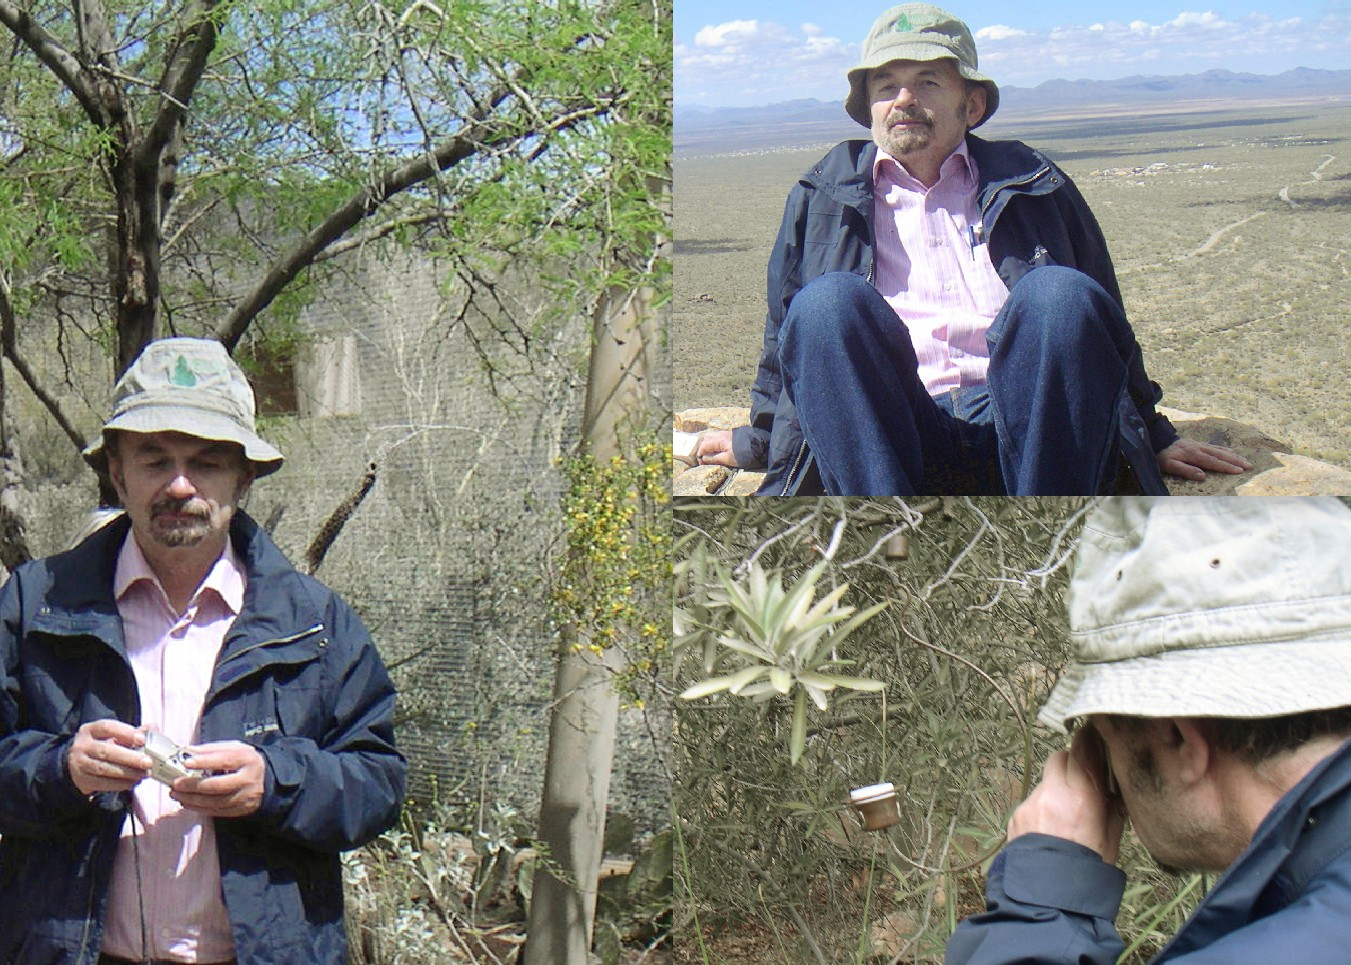
\includegraphics[width=0.95\columnwidth]{07March24HaraldCollageDesertMuseum.jpg}}
\caption{Harald Fritzsch visiting Arizona-Sonora Desert Museum in Spring 2007. Pictures and picture assembly by Johann Rafelski
}
\label{Fig:AZcolloq2007} 
\end{figure}

These meetings offered an opportunity to exchange ideas the  origin of neutrino mass and parameters of  the standard model were close to his heart. Were these parameters really natural constants on cosmological time scale? In Figure\,\ref{Fig:RANP2004} we see Harald's first transparency ``Time Dependence of QCD and Experimental Tests'' made at at the 9th Hadron Physics and 7th Relativistic Aspects of Nuclear Physics (HADRON-RANP 2004): A Joint Meeting on QCD and QGP: Rio de Janeiro, Brazil, March 28-April 3, 2004~\cite{Fritzsch:2004civ}, a meeting we both attended. We see that Harald modified slightly by hand the typed transparency to introduce the meeting specific context in a talk which arose from another publication of the epoch, Ref.\,\cite{Calmet:2001nu}. 

\begin{figure}%[ht]
\centerline{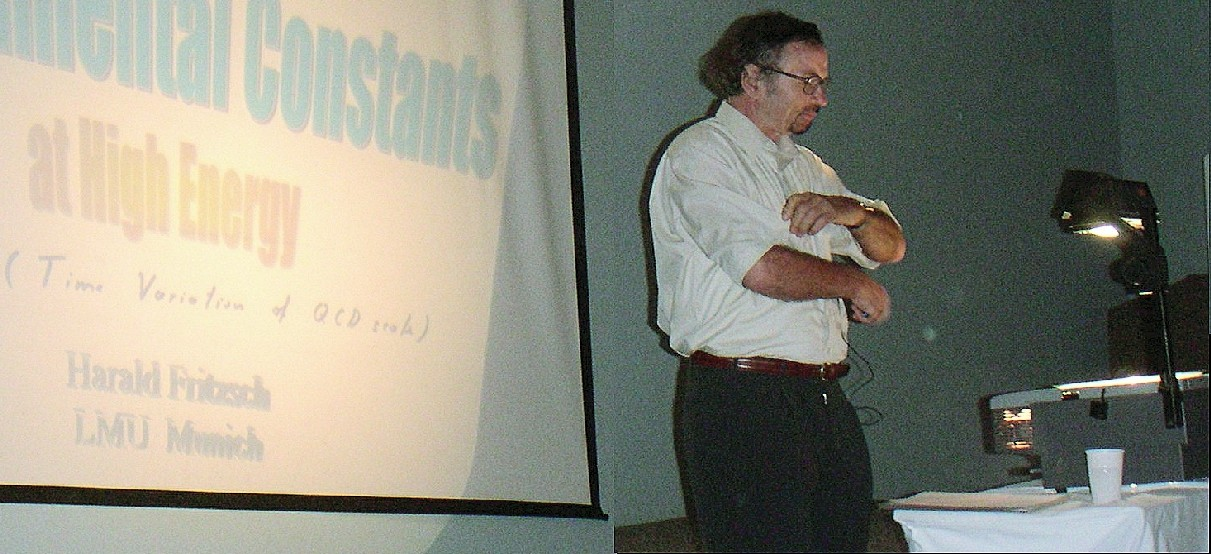
\includegraphics[width=0.95\columnwidth]{04RANPHarald1Ed.jpg}}
\caption{Harald begins his presentation in Rio de Janeiro 2004 about time dependence of QCD, see text for details. Picture by Johann Rafelski
}
\label{Fig:RANP2004} 
\end{figure}
 
%%%%%%%%%%%%%%%%%%%%%%%%%%%%%%%%%%%%


\bibliographystyle{ws-rv-van}
\bibliography{Rafelski_Steinmetz_for_Harald}
%%%%%%%%%%%%%%%%%%%%%%%%%%%%%%%%%%%%
\end{document} 
%%%%%%%%%%%%%%%%%%%%%%%%%%%%%%%%%%%%
